\documentclass{article}[12pt]

%--------------Packages------------------------------
\usepackage[utf8]{inputenc} %Pour encoder du texte en français
\usepackage[francais]{babel} %Pour encoder du texte en français
\usepackage{graphicx} %pour inclure des images
\usepackage{changepage}
\usepackage{version} % permet d'utiliser l'environnement comment
\graphicspath{{./figures/}} %repertoire images
\usepackage{listings} %si on veut afficher du code, le code doit se trouver dans un dossier "codes" 					  %lui même dans le même répertoire que ce fichier tex
\usepackage{color} %nécessaire pour changer les couleurs du highlighting du code
\usepackage{amsmath,amssymb}%pour des maths au cas où
\usepackage{array,multirow,makecell}%Pour manipuler les tableaux
\usepackage{url} %pour utiliser les liens hypertextes
\usepackage{hyperref} %pour utiliser les liens hypertextes
\usepackage{float}
\newlength{\offsetpage}
\setlength{\offsetpage}{2.0cm}
\newenvironment{widepage}{\begin{adjustwidth}{-\offsetpage}{-\offsetpage}%
    \addtolength{\textwidth}{2\offsetpage}}%
{\end{adjustwidth}}

\newcommand{\JavaScript}[2]{
	\begin{itemize}
		\item[]\lstinputlisting[caption=#2,label=#1]{#1.js}
	\end{itemize}
}
% ---------- Document ------------ %
\begin{document}

\begin{titlepage}

\newcommand{\HRule}{\rule{\linewidth}{0.5mm}} % Defines a new command for the horizontal lines, change thickness here

\center % Center everything on the page
 
%----------------------------------------------------------------------------------------
%	HEADING SECTIONS
%----------------------------------------------------------------------------------------

\textsc{\LARGE Institut Paul Lambin}\\[1.5cm] % Name of your university/college
\textsc{\Large BAC 2 Informatique de gestion}\\[0.5cm] % Major heading such as course name
\textsc{\large Unix}\\[0.5cm] % Minor heading such as course title

%----------------------------------------------------------------------------------------
%	TITLE SECTION
%----------------------------------------------------------------------------------------

\HRule \\[0.4cm]
{ \huge \bfseries Synthèse Unix }\\[0.4cm] % Title of your document
\HRule \\[1.5cm]
 
%----------------------------------------------------------------------------------------
%	AUTHOR SECTION
%----------------------------------------------------------------------------------------

\begin{minipage}{0.4\textwidth}
\begin{flushleft} \large
\emph{Auteurs:}\\
Christopher \textsc{Sacré} \\ % Your name
\end{flushleft}
\end{minipage}
~
\begin{minipage}{0.4\textwidth}
\begin{flushright} \large
\emph{Professeur:} \\
C. \textsc{De Muylder}\\
B. \textsc{Henriet}\\
A. \textsc{Ninane}% Supervisor's Name

\end{flushright}
\end{minipage}\\[4cm]

% If you don't want a supervisor, uncomment the two lines below and remove the section above
%\Large \emph{Author:}\\
%John \textsc{Smith}\\[3cm] % Your name

%----------------------------------------------------------------------------------------
%	DATE SECTION
%----------------------------------------------------------------------------------------

{\large \today}\\[3cm] % Date, change the \today to a set date if you want to be precise

%----------------------------------------------------------------------------------------
%	LOGO SECTION
%----------------------------------------------------------------------------------------

%\includegraphics{Logo}\\[1cm] % Include a department/university logo - this will require the graphicx package
 
%----------------------------------------------------------------------------------------

\vfill % Fill the rest of the page with whitespace

\end{titlepage}

\tableofcontents%table des matières
\newpage

\section{Présentation du JavaScript}

\subsection{Langage d'avenir}

Le JavaScript est un langage créé pour le front-end Web, il peut également être utilisé au niveau back-end Web notamment à l'aide de Node.js.

\subsection{Mauvaise réputation}

\paragraph{Argument 1} : Performances médiocres

\paragraph{Argument 2} : Le langage est considéré comme sale, ceci est du à certaines {\color{blue}spécificités} du langage parfois inhabituelles. ({\color{blue}Beaucoup de manières de faire la même chose}, et ceci de manière très différentes).

\subsection{Les bons côtés}

Il existe divers moyens afin de réaliser la même opération et de ce fait parmi toutes ces manières, il en existe forcément {\color{blue} une simple à comprendre et à utiliser} 

\subsection{Langage interprété}

Il n'y a pas de phase de compilation, c'est donc le code source qui sera directement utilisé lors de la compilation.

\subsection{Langage dynamiquement typé}

Le type des variables est déterminé à l'exécution, le mot clef {\color{blue} var} sert à déclarer les variables (Attention, le type d'une variable peut changer lors de l'exécution du programme).
\newpage
\subsection{Opérateur instanceOf}

\begin{figure}[H]
	\centering
	\fbox{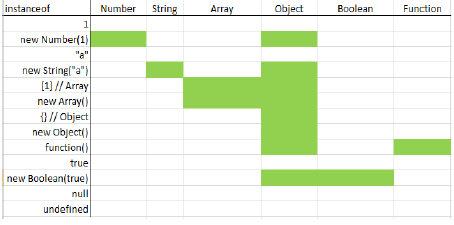
\includegraphics{instanceOf.PNG}}
    \caption{Tableau montrant le résultat renvoyé par l'opérateur instanceOf}
\end{figure}

\subsection{Opérateur typeOf}

Fonction permettant de tester une variable et de retourner une chaîne de caractères décrivant le type de cette dernière.

\begin{figure}[H]
	\centering
	\fbox{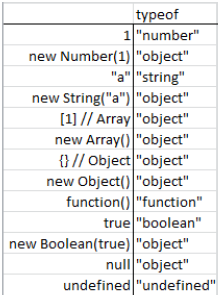
\includegraphics[scale=0.90]{typeOf.PNG}}
    \caption{Tableau montrant le résultat renvoyé par l'opérateur typeOf}
\end{figure}

\subsection{Différence entre "==" et "==="}

"==" effectue un transtypage faiblement typé. Ceci peut parfois donner des résultats surprenant, on évitera donc de l'utiliser. équivalent de "==" pour démontrer une inégalité : "!="
\newline
\newline
"===" n'effectue pas de transtypage, on le privilégiera donc à "==",  équivalent de "===" pour démontrer une inégalité : "!==".

\subsection{Les fonctions}

Une fonction est considéré comme une méthode sans classe, par ailleurs les fonctions peuvent très bien être assignées au sein de variables. 
\newline
\newline
Étant donné qu'une fonction peut etre affectée à des variables de noms différents, le nom de la fonction n'a pas réellement d'importance. Dans certains cas on ne nommera même pas la fonction (elle sera donc considérée comme une fonction anonyme)
\newline
\newline
C'est la présence ou l'absence de parenthèses qui détermine si on parle de la référence de la fonction, ou de son exécution.

\subsection{Portée lexicale des variables}

Une variable ne se restreint pas au bloc où elle est déclarée, elle se restreint plutôt à la fonction qui  l'englobe.
\newline
\newline
Il faut faire attention aux variables globales car si celles sont utilisées pour définir une autre variable ce sera la référence de la variable globale qui sera retenue au sein de celle-ci et non sa valeur.

\subsection{OO en JavaScript}

JavaScript supporte aussi la programmation orientée objet, mais la manière dont elle fonctionne est fortement différente du java.
\newline
\newline
Les Objets JavaScript indépendamment de la programmation OO fonctionne comme des Maps. On associe une clé à une valeur, on parle alors d'objets associatifs.

\subsection{Gestion des attributs}

\JavaScript{attribute_value}{Valeur d'un attribut}
\JavaScript{change_value}{Modification d'un attribut}
\JavaScript{delete_value}{Suppresion d'un attribut}

\subsection{Objets et héritages}

Les attributs d'un objet peuvent provenir d'un parent de l'objet, par contre la méthode Object.keys ne renverra pas les attributs parents, si l'on désire tout de même y accéder on peut toujours utiliser un for(... in ...). On peut également savoir si un objet possède un attribut a l'aide de la méthode hasOwnProperty("attribut").

\subsection{Pseudo Classe}

\JavaScript{decla_pseudo_classe}{Exemple de déclaration d'une pseudo classe}

\JavaScript{util_pseudo_classe}{Exemple d'utilisation d'une pseudo classe}

\JavaScript{heritage}{Exemple d'utilisation de l'héritage sur une pseudo classe}

\section{JavaScript dans le browser}

\subsection{Ajout du JavaScript au sein de notre page HTML}

\JavaScript{ajoutJS_direct}{Directement au sein de la page HTML}

\JavaScript{ajoutJS_indirect}{Au sein d'un fichier séparé du reste de la page HTML}

\subsection{Méthodes / Variables utiles}

\begin{itemize}
	\item console.log : affiche au sein de la console ce qui lui est passé en paramètre (si variable affiche son contenu).
    \item navigator : objet contenant de l'information sur le browser lui-même, permet de l'identifier.
    \item window : objet manipulant la fenêtre du browser.
    \item document : objet manipulant la fenêtre du browser (document.writeln("argument") remplace le contenu de la pge HTML par celui passé en paramètre).
    \item location : objet représentant l'URL de la page.
    (location.href = cette URL, location.reload() recharge la page, location.replace("URL") navigue vers l'url passée en paramètre).
\end{itemize}
\newpage
\subsection{Document Object Model (DOM)}

\subsubsection{Présentation générale du DOM}

Le navigateur crée de lui même une représentation objet de la page. Lorsque cet objet est manipulé par JavaScript, ce dernier se mets automatiquement à jour.
\newline
\newline
Le DOM a une structure en arbre où chaque nœud représente un élément HTML, par ailleurs certains attributs correspondent aux attributs HTML. Certaines fonctions permettent de manipuler de diverses manières le nœud et/ou d'accéder 	aux autres nœuds.
\newline
\newline
En pratique, traverser un arbre pour trouver un nœud en particulier est très peu souple  (Si on change la moindre chose dans notre structure HTML on devra modifier l'intégralité de notre code en conséquence. Il existe donc des raccourcis facilitant l'accès à des nœuds en particulier.
\begin{figure}[H]
	\centering
    \fbox{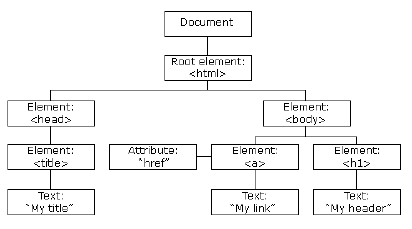
\includegraphics{dom.PNG}}
    \caption{Exemple de représentation du DOM d'une page HTML}
\end{figure}

\subsubsection{Quelques méthodes utiles du DOM}
\begin{itemize}
	\item \emph{document.getElementById(...)} : retourne l'objet portant l'id entré en paramètre
    \item \emph{document.getElementsByName(...) } : retourne les objets ayant l'attribut name égal à celui passé en paramètre. (Cette méthode renvoie donc un tableau d'éléments).
    \item \emph{document.getElementsByClassName(...)} : retourne les objets ayant une classe css égale à celle passée en paramètre de la méthode).
    \item \emph{document.getElementsByTagName(...)} : retourne les objets dont le tag HTML est équivalent à celui entré en paramètre.
\end{itemize}

\subsection{Les événements}

Les événements 	permettent de pouvoir réagir aux actions de l'utilisateur, on enregistre alors les fonctions qui seront appelées lors d'actions spécifiques de l'utilisateur (action utilisateur = un événement sur un élément du DOM).
\newline
\newline
Les éléments HTML possèdent des attributs affectables à une fonction JavaScript.
\begin{figure}[H]
	\centering
    \fbox{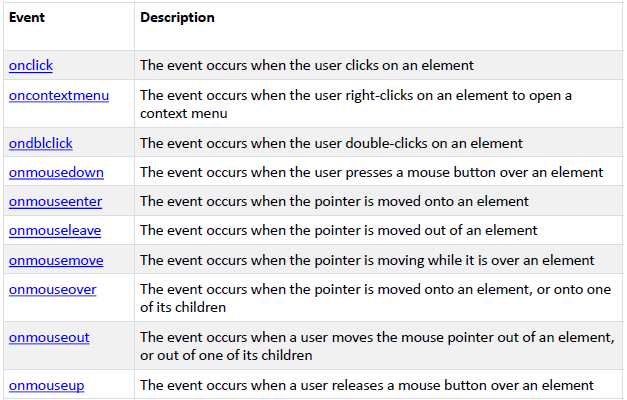
\includegraphics[scale=0.90]{event_souris.PNG}}
    \caption{Pour exemple voici les événements rattachés à la souris}
\end{figure}
 Par contre, la valeur de l'attribut est unique, si on change cette valeur, la fonction précédemment affectée à cet événement ne sera plus appelée. L'HTML peut quant à lui référencé une fonction JavaScript qui n'est pas encore chargée, Ceci peut conduire a certains disfonctionnements si l'utilisateur réagit trop vite. (Afin de se prévenir de ces problèmes, on enregistre via le DOM, \emph{document.body.addEventListener("click", function(){}})).
\newline
\newline
Les navigateurs ne permettent d'effectuer qu'une seule tâche à la fois (on dit qu'ils sont monothreadés). Ainsi, quand le JS s'exécute, rien d'autre ne s'exécute (pas de chargement de page, pas de rafraîchissement de la page, pas d'autres JS, pas d'interactions avec l'utilisateur, ...).
\newline
\newline
Cas spécial, la fonction : \emph{setTimeout(f,t)}, utilisée si l'on souhaite effectuer des actions dans le futur, .., f sera une fonction appelée après t millisecondes. (Il existe une alternative si l'on désire créer un intervalle : \emph{setInterval(f,t)}

\section{Lecture optionnelle mais conseillée}
\end{document}